% Release MA_ROPE_TVT_v24_PureSim_20261014-1223_LATEST - generated by release.sh from main.tex + sections/tables/figures
\documentclass[journal,10pt,twocolumn]{IEEEtran}
\usepackage{amsmath,amsfonts,amssymb}
\usepackage{graphicx}
\usepackage{booktabs}
\usepackage{tabularx}
\usepackage{tikz}
\usetikzlibrary{arrows.meta,shapes.geometric,shapes.symbols,calc}
\usepackage{multirow}
\usepackage{siunitx}
\usepackage{cite}
\usepackage[hidelinks]{hyperref}
\usepackage{cleveref}
\usepackage{algorithm}
\usepackage{algorithmic}

\flushbottom
\begin{document}

\title{Multi-RAT Privacy-Preserving Federated Deep Reinforcement Learning for V2X Task Offloading}
% \author{...}  % author names/affiliations to be added by the authors

\maketitle

\begin{abstract}
Autonomous vehicles increasingly run computation-heavy tasks with strict service-quality demands that their onboard processors cannot always meet on their own, which is why offloading part of that work to the network edge has become common practice. When many vehicles compete for the same wireless link and the same edge server, however, a policy that offloads aggressively without regard for channel conditions or queue congestion can fail badly, and this failure mode is easy to miss if a system is only ever tested at one vehicle density. This paper presents MA-ROPE, a Multi-RAT (Radio Access Technology) Privacy-Preserving Federated Deep Reinforcement Learning framework for Vehicle-to-Everything (V2X) task offloading. MA-ROPE jointly chooses among four radio interfaces (LTE, ITS-G5, Wi-Fi 6, and 5G-NR) and decides how much of each task to offload, using a Dueling Double Deep Q-Network (D3QN) whose training is coordinated across vehicles through Federated Averaging (FedAvg) so that raw training observations are not pooled across vehicles (the offloaded share of a task is still sent to the RSU). Under dense, latency-critical traffic, MA-ROPE significantly improves the rate at which tasks are completed on time compared to fixed single-radio baselines. We also introduce the Deadline Retention Ratio, a new metric for how much of a policy's on-time performance survives a large increase in fleet size, and find that MA-ROPE holds onto nearly all of its performance while baseline methods experience severe degradation. Furthermore, the joint radio-selection and offloading logic adds no measurable computational overhead over simpler controllers. Ultimately, radio selection, partial offloading, and edge-queue contention must be optimized jointly, not separately, for vehicular networks to deliver time-critical tasks reliably as they scale.
\end{abstract}
\begin{IEEEkeywords}
Task offloading, Vehicle-to-Everything (V2X) communication, vehicular edge computing, federated deep reinforcement learning, multi-RAT selection, heterogeneous networks, edge computing, autonomous driving, privacy-preserving learning, Jakes fading.
\end{IEEEkeywords}

\section{Introduction}

Vehicle-to-Everything (V2X) communication enables safety-critical and compute-intensive applications such as cooperative perception, autonomous driving, and real-time hazard avoidance. These applications impose heterogeneous Quality-of-Service (QoS) requirements: safety messages may become unusable within approximately 100 ms, whereas compute and infotainment workloads can tolerate substantially larger delays. At the same time, processing the growing volume of camera, radar, and LiDAR data entirely on resource-constrained vehicle Electronic Control Units (ECUs) is increasingly difficult. Vehicular Edge Computing (VEC) addresses this limitation by offloading computation to roadside Multi-access Edge Computing (MEC) servers.

The effectiveness of offloading, however, depends jointly on where computation is performed and how the offloaded workload reaches the edge. No single Radio Access Technology (RAT) is uniformly optimal across task types and mobility conditions. Long-Term Evolution (LTE), ITS-G5 (the European Intelligent Transport Systems band at 5.9 GHz), WiFi-6, and 5G New Radio (5G-NR) exhibit different latency, throughput, coverage, and mobility characteristics. A RAT suitable for a delay-tolerant compute task may therefore be unsuitable for a safety-critical task generated by the same vehicle. Moreover, binary local/offload decisions cannot exploit parallel local and MEC processing. These observations motivate treating RAT selection and partial computation offloading as a joint decision rather than as independent optimization stages.

A second challenge emerges as vehicle density increases. Vehicles associated with the same Roadside Unit (RSU) compete not only for wireless resources but also for a shared MEC processing queue. Consequently, aggressive offloading that performs well for an isolated vehicle may degrade when many vehicles simultaneously submit workloads. This degradation can also be hidden by conventional communication metrics. Packet Reception Ratio (PRR) counts a packet as successfully delivered even when it arrives after its application deadline; for safety-critical traffic, however, a late result may be operationally equivalent to a lost one. Evaluation must therefore distinguish successful reception from deadline-compliant delivery.

To address these coupled challenges, we propose MA-ROPE, a multi-agent framework that jointly learns RAT selection and partial computation offloading under shared MEC contention. The core insight is that RAT choice and offload ratio are mutually dependent: the selected RAT determines transmission latency and reliability, which in turn determines the feasible offload ratio; conversely, the offload ratio sets transmission duration, which affects queue contention and RSU delay for all co-located vehicles. Optimizing these decisions sequentially yields suboptimal policies because downstream interactions are ignored.

Each vehicle selects among LTE, ITS-G5, WiFi-6, and 5G-NR while adapting its offloaded workload fraction $\rho \in \{0.25, 0.50, 0.75, 1.0\}$ to channel conditions, task requirements, energy budget, and current RSU queue state. The MDP state explicitly includes shared queue depth $Q$, enabling each vehicle's policy to account for the decisions of co-located vehicles. A Dueling Double Deep Q-Network (D3QN) decomposes value and advantage streams, enabling stable learning under multi-vehicle interactions. Federated Averaging (FedAvg) coordinates policies across vehicle clusters without requiring vehicles to share raw observations, preserving operational privacy while enabling cooperative learning at the policy level.

Accordingly, this work investigates whether a federated multi-RAT offloading policy can preserve deadline-compliant V2X delivery as fleet density and shared MEC contention increase.

Despite extensive research on VEC offloading, existing approaches generally address only subsets of heterogeneous RAT selection, partial computation offloading, multi-vehicle MEC contention, mobility-aware channel behavior, and federated cooperative learning. Recent distributed deep RL methods (e.g., \cite{zhao2024}, \cite{guo2026}) employ federated learning or game-theoretic coordination, but typically optimize RAT selection or offload ratio independently, rather than jointly. Bandit-based approaches (e.g., \cite{haq2026}) adapt network selection to density, but do not model partial execution or shared queue dynamics. Task-splitting strategies (surveyed in \cite{mach2017}) typically rely on analytical optimization rather than learning from channel variability and queue state. The closest prior work we are aware of, Xiong et al.~\cite{xiong2021}, combines heterogeneous V2X access technologies with federated Q-learning for task offloading. We do not claim that this combination is new; our contribution is the joint (RAT, offload-ratio) decision space under a shared RSU backlog and the evaluation of deadline retention across fleet densities.

MA-ROPE addresses this gap by bringing these dimensions together and introducing a new evaluation discipline: not only performance at a fixed operating point, but critically, how well deadline-compliant service survives increasing fleet contention. We quantify this via the Deadline Retention Ratio (DRR), which measures how much of a policy's reference-density on-time performance remains at higher densities. This metric reveals that aggressive offloading policies that perform well at low vehicle density can collapse catastrophically as the fleet grows, a failure mode invisible to scalar operating-point metrics.

The main contributions of this work are:


First, we formulate RAT selection and partial computation offloading as a unified MDP decision, not as sequential stages. Unlike prior work that selects the RAT first and then optimizes offload ratio (or vice versa), we model the action space as (RAT, $\rho$) pairs, directly encoding the mutual dependence. Critically, the MDP state includes the shared RSU queue depth, enabling each vehicle to account for others' decisions and avoid the "AllOffload collapse" observed when vehicles naively offload all traffic without considering queue saturation.
Second, We coordinate D3QN training across vehicle clusters via Federated Averaging (FedAvg), enabling cooperative learning without centrally pooling raw vehicle observations. The key innovation is that the per-agent state explicitly includes the shared RSU queue depth, making each vehicle's learned policy aware of co-located vehicle demand. This differs from pure distributed RL by incorporating shared resource constraints at the agent level, not requiring a central coordinator during execution.
Third, We distinguish communication reliability (PRR) from application-useful on-time delivery (OTR). We introduce the DRR, which normalizes a policy's on-time delivery at a target density relative to its own reference-density performance, enabling fair comparison across heterogeneous policies without dependence on utility-function constants.
Finally, We evaluate MA-ROPE and four baselines across multiple fleet sizes ($N \in \{8, 16, 32\}$) under URLLC traffic. We demonstrate that while baseline policies suffer catastrophic failure modes at high contention, the proposed federated MDP formulation robustly maintains deadline compliance, link reliability, and low computational overhead across varying densities.


\section{Related Work}

\subsection{Task Offloading in Vehicular Networks}

Existing V2X offloading approaches broadly include heuristic, optimization-based, and learning-based methods. Greedy and heuristic schemes select offloading destinations using predefined decision rules, but their ability to adapt to rapidly varying channel conditions and shared-resource contention is limited. Bandit and tabular approaches such as UCB~\cite{auer2002} introduce online adaptation but are better suited to relatively small and stationary decision spaces. Control-theoretic methods based on Lyapunov optimization~\cite{mao2016} explicitly address queue stability, but generally optimize time-averaged objectives rather than task-specific deadline compliance. Deep Reinforcement Learning (DRL) approaches~\cite{xiong2021,lowe2017} provide greater adaptability, although many existing formulations simplify either the communication interface or the computation decision through single-RAT operation or binary local/offload actions.

Guo et al.~\cite{guo2026} proposed DTOF/HIOA, combining a Double DQN with a Long Short-Term Memory (LSTM) network and Nash-equilibrium-based optimization in a three-tier cloud-edge-vehicle architecture over 5G-NR. Although the framework achieves strong delay performance, it does not jointly consider heterogeneous RAT selection, federated cooperation, and shared RSU queue contention across co-located vehicles.

A complementary line of work considers partial offloading, where a task is divided between local and MEC execution rather than being processed entirely at one location. Parallel local and remote execution can reduce completion time by exploiting both computing resources simultaneously. Prior work has established such parallel-execution models~\cite{mach2017}, including formulations in which total completion delay is governed by the slower of the local and remote processing branches. In most such approaches, however, the offload ratio is optimized independently of heterogeneous radio selection. MA-ROPE instead couples these decisions: the amount of computation transmitted and the RAT used for transmission are jointly determined, with the realized offload ratio adapting to the SINR of the selected interface.

\subsection{Multi-RAT and Heterogeneous Access Selection}

Heterogeneous V2X access has traditionally been studied primarily as a communication-selection problem. Yacheur et al.~\cite{yacheur2023} developed Double DQN based selection between ITS-G5 and LTE-V2X, demonstrating the benefit of adapting RAT choice to channel conditions. Their physical-layer parameters and SINR-based Division Mode motivate elements of the heterogeneous channel and partial-offloading models adopted in MA-ROPE.

More recent work has expanded heterogeneous access beyond two interfaces, with studies considering multi-RAT assignment and heterogeneous V2X resource allocation across combinations such as Dedicated Short-Range Communications (DSRC), cellular V2X, and millimeter-wave (mmWave) links. Mirza et al.~\cite{mirza2023} proposed the Mobility, Contact, and computational Load-Aware (MCLA) task offloading framework for heterogeneous 5G-NR-V2X edge networks, incorporating mobility, contact duration, MEC load awareness, and task partitioning. Their scheme supports load-aware server selection and partial execution, but uses model-based decision logic rather than a learned federated joint RAT-offload policy.

These studies establish the value of heterogeneous access, but their decision structures remain different from the problem addressed here. RAT-selection methods generally determine the interface over which an already-defined workload is transmitted, whereas computation offloading must additionally determine how much workload should be transmitted. The two decisions interact directly because the selected RAT affects transmission latency and reliability, while the offloaded fraction determines transmission duration, energy consumption, local computation demand, and MEC load.

MA-ROPE therefore represents RAT identity and workload partitioning within a common decision process rather than optimizing them as separate stages.

\subsection{Federated and Privacy-Preserving Learning for VEC}

Cooperative learning has increasingly been applied to vehicular edge resource management. Centralized multi-agent approaches such as Multi-Agent Deep Deterministic Policy Gradient (MADDPG)~\cite{lowe2017} can exploit joint agent information during training and provide strong coordination, but require centralized access to information that remains local under a federated formulation.

Federated learning offers an alternative by aggregating model parameters rather than centrally collecting each vehicle's training observations. Moon and Lim~\cite{moonlim2022} proposed federated Deep Deterministic Policy Gradient (DDPG) learning for vehicular edge task offloading and power control, combining local actor-critic learning with periodic model aggregation. Their formulation incorporates queue information and power control, but does not perform heterogeneous RAT selection or explicit partial-offload-ratio selection. Other recent federated VEC approaches employ Double Deep Q-Network (DDQN) methods or multi-agent DRL with FedAvg for collaborative offloading, but similarly focus on destination or mode selection rather than a joint RAT-partial-offload action.

Accordingly, the contribution of MA-ROPE is not simply the combination of federated learning and multi-RAT access. Rather, FedAvg is applied to a policy whose decision space jointly captures heterogeneous RAT selection, workload partitioning, and queue-aware offloading.

The privacy benefit should also be interpreted carefully. FedAvg avoids centralized pooling of raw observations, but exchanging model updates does not itself provide formal privacy guarantees because trained parameters may remain vulnerable to inference attacks~\cite{zhu2019}. Secure aggregation and differential privacy are therefore complementary mechanisms for production deployment.

\subsection{Research Gap and Positioning}

The literature demonstrates substantial progress in each component of vehicular edge offloading, but these components are predominantly addressed in isolation. We position MA-ROPE against the most closely related recent works across several dimensions. Federated multi-agent DRL for VEC has been proposed for task offloading, combining local actor-critic learning with periodic model aggregation~\cite{zhao2024}. However, such formulations often do not perform heterogeneous RAT selection or model explicit partial-offload-ratio choice. Similarly, combining federated DDPG with queue information~\cite{moonlim2022} lacks optimization over heterogeneous RATs or joint RAT-$\rho$ decisions.

Multi-RAT offloading under distributed learning has also been explored, such as heterogeneous V2X offloading with federated Q-learning~\cite{xiong2021} or cloud-edge-vehicle offloading with game theory~\cite{guo2026}. These works address RAT diversity and distributed learning; our emphasis differs in the joint (RAT, $\rho$) action space, the shared RSU backlog, and the quantification of how deadline-compliant delivery is retained as fleet density grows.

Density-aware network selection using bandit-based and heuristic approaches~\cite{haq2026} adapts network selection to vehicle density, but operates in a lower-complexity decision space and typically assumes fixed offload destinations. Task splitting and fairness constraints have been modeled by optimization-based approaches~\cite{mach2017}, but these rely on analytical solutions rather than learning from channel variability, and do not address the adaptive multi-RAT selection problem.

MA-ROPE differs from each of these in that it (1) jointly optimizes RAT selection and partial offload ratio within a unified MDP, (2) explicitly models shared RSU queue contention in the agent state to avoid naive all-offload policies, and (3) introduces and evaluates the Deadline Retention Ratio across multiple fleet densities—a metric absent from prior work. Table I summarizes the positioning of MA-ROPE relative to representative prior approaches.

\begin{table*}[t]
\caption{Literature Comparison: Feature Coverage. FL: Federated Learning. ``--'': not assessed.}
\label{tab:literature}
\centering
% booktabs-restyled
\footnotesize
\setlength{\tabcolsep}{3pt}
\renewcommand{\arraystretch}{1.15}
\begin{tabularx}{\textwidth}{>{\hsize=1.132\hsize\raggedright\arraybackslash}X>{\hsize=1.029\hsize\centering\arraybackslash}X>{\hsize=0.926\hsize\centering\arraybackslash}X>{\hsize=1.029\hsize\centering\arraybackslash}X>{\hsize=1.029\hsize\centering\arraybackslash}X>{\hsize=0.824\hsize\centering\arraybackslash}X>{\hsize=1.029\hsize\centering\arraybackslash}X}
\toprule
\textbf{Paper} & \textbf{Multi-RAT} & \textbf{Partial $\rho$} & \textbf{Queue Cont.} & \textbf{FL Privacy} & \textbf{Jakes} & \textbf{Yacheur Ch.} \\
\midrule
Guo 2026~\cite{guo2026} & $\times$ & Partial & Per-node & $\times$ & $\times$ & $\times$ \\
Yacheur 2023~\cite{yacheur2023} & \checkmark ITS+LTE & $\times$ & $\times$ & $\times$ & \checkmark & \checkmark \\
Xiong 2021~\cite{xiong2021} & \checkmark 3 RATs & -- & -- & \checkmark federated Q & -- & -- \\
\textbf{MA-ROPE (ours)} & \textbf{\checkmark 4 RATs} & \textbf{\checkmark $\rho\in\{0..1\}$} & \textbf{\checkmark shared RSU} & \textbf{\checkmark FedAvg} & \textbf{\checkmark Jakes} & \textbf{\checkmark adopted} \\
\bottomrule
\end{tabularx}
\end{table*}



\section{System Model and Problem Formulation}

\subsection{Network Architecture}

We consider a two-tier V2X network comprising N vehicles, R roadside units (RSUs) each co-located with a MEC server, and a base station (BS) providing wide-area LTE and 5G-NR coverage. Each vehicle has an on-board ECU capable of 2-5 Tera Operations Per Second (TOPS) and a multi-RAT module supporting LTE, ITS-G5, WiFi-6, and 5G-NR simultaneously. \Cref{fig:network_topology} illustrates the system architecture.

\begin{figure*}[t]
\centering
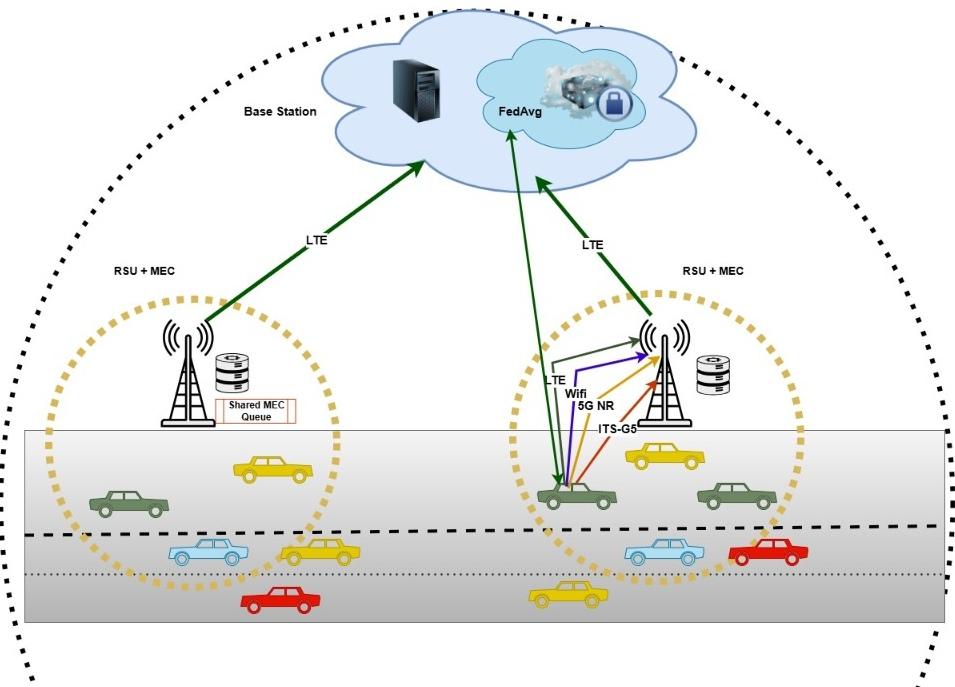
\includegraphics[width=0.78\textwidth]{figures/fig3_network_topology.jpg}
\caption{Network topology with 4-RAT heterogeneous access and FedAvg coordination.}
\label{fig:network_topology}
\end{figure*}


\subsection{RAT Physical Layer Model}

Following Yacheur et al.~\cite{yacheur2023}, we assign per-RAT physical parameters as in \Cref{tab:rat_physical}. LTE and 5G-NR operate at -110 dBm noise floor; ITS-G5 and WiFi-6 at -90 dBm. Cellular RATs experience Jakes Doppler fading at vehicular speeds; ITS-G5 and WiFi-6 use the Constant Speed propagation model, as analyzed in \Cref{fig:jakes_fading}.

\begin{table*}[t]
\caption{RAT Physical Parameters (Yacheur 2023 + 3GPP Standards)}
\label{tab:rat_physical}
\centering
% booktabs-restyled
\footnotesize
\setlength{\tabcolsep}{3pt}
\renewcommand{\arraystretch}{1.15}
\begin{tabularx}{\textwidth}{>{\hsize=1.474\hsize\raggedright\arraybackslash}X>{\hsize=0.921\hsize\centering\arraybackslash}X>{\hsize=0.921\hsize\centering\arraybackslash}X>{\hsize=0.921\hsize\centering\arraybackslash}X>{\hsize=0.921\hsize\centering\arraybackslash}X>{\hsize=0.921\hsize\centering\arraybackslash}X>{\hsize=0.921\hsize\centering\arraybackslash}X}
\toprule
\textbf{RAT} & \textbf{Delay} & \textbf{Throughput} & \textbf{Noise Floor} & \textbf{Fading} & \textbf{Path Loss} & \textbf{Source} \\
\midrule
LTE & 20 ms & 50 Mbps & -110 dBm & Jakes & TR 36.885 & \cite{yacheur2023} \\
ITS-G5 & 10 ms & 27 Mbps & -90 dBm & Constant & TR 36.885 & \cite{yacheur2023} \\
WiFi-6 & 5 ms & 600 Mbps & -90 dBm & Constant & 802.11ax & \cite{ieee80211ax} \\
5G-NR & 1 ms & 1 Gbps & -110 dBm & Jakes & TR 38.901 & \cite{3gpp2022} \\
\bottomrule
\end{tabularx}
\end{table*}


The Signal-to-Interference-plus-Noise Ratio (SINR) for RAT $r$ at distance $d$ with vehicle speed $v$ governs per-PDU delivery probability:

\begin{equation}
\label{eq:sinr}
\text{SINR}_r(d,v) = P_{tx} - \text{PL}_r(d) - N_r - Sh_r - F_r(v)
\end{equation}

where $\text{PL}_r(d)$ is RAT-specific path loss, $N_r$ is noise floor, $Sh_r \sim \mathcal{N}(0,\sigma^2_r)$ is shadowing, and $F_r(v)$ is Jakes fading loss. SINR drives a per-PDU Bernoulli draw with $p_{link} = \sigma(\text{SINR}_r - \theta_r)$ but is NOT the reported PRR metric. Packet Reception Ratio is defined empirically from actual packet counters:

\begin{equation}
\label{eq:prr}
\text{PRR} = \frac{n_{rx}}{n_{tx}}
\end{equation}

where $n_{tx}$ is the number of offload PDU transmission attempts and $n_{rx}$ is PDUs successfully delivered. This separates the physical link model from the reported metric: PRR reflects real packet outcomes, not a smoothed SINR function. Per-RAT empirical PRR fills observation slots obs[4:8]; slots default to 0.5 (unknown) before any attempt on that RAT. The raw link delivery probability $p_{link}$ is separately tracked in infos["link\_delivery\_prob"] for comparing the physical-layer (PHY) curve against measured PRR.

\subsection{Task Model}

Each vehicle generates task $\tau_i = (C_i, V_i, D_i, T_i)$ where $C_i$ is computational workload (CPU cycles), $V_i$ is data volume (MB), $D_i$ is the task's deadline, its maximum tolerable delay (ms), and $T_i \in \{\text{safety}, \text{infotainment}, \text{compute}\}$ determines that deadline: safety tasks require $D_i = 100$ ms (e.g., 3GPP TR 36.885~\cite{molina2017}), infotainment 500 ms, compute 2000 ms.

A vehicle may partition task $\tau_i$ into local and remote execution fractions, parameterized by the offload ratio $\rho \in [0, 1]$:
\begin{equation}
\label{eq:offload_ratio}
C_{\text{local}} = (1 - \rho) \cdot C_i, \quad C_{\text{remote}} = \rho \cdot C_i,
\end{equation}
where $\rho = 0$ denotes fully local execution and $\rho = 1$ denotes full offloading to the MEC server.

\subsection{End-to-End Latency Model}

End-to-end task latency is the primary measurable QoS quantity in this work. For each offload PDU attempt at step t, the total latency decomposes into six additive components:

\begin{subequations}
\label{eq:latency_all}
\begin{equation}
\label{eq:ltotal_base}
L_{total} = L_{prop} + L_{tx} + L_{queue} + L_{remote} + L_{rx} + L_{prop}
\end{equation}

where $L_{prop} = d/(2c/3)$ is propagation delay over vehicle-to-RSU distance d at 2/3 speed of light; $L_{tx} = V_i/\text{BW}_r$ is uplink transmission delay for data volume $V_i$ (MB) over RAT bandwidth $\text{BW}_r$; $L_{remote} = C_i/f_{MEC}$ is remote compute delay for workload $C_i$ (CPU cycles) at MEC frequency $f_{MEC}$; $L_{rx}$ is the downlink reception delay for the computed results; and $L_{queue} = \tau\,Q_r$ is the queueing delay at the shared RSU $r$, where $Q_r$ is the offload backlog, the sum of the offload ratios requested by all vehicles served by RSU $r$ in the current step, and $\tau = 50$ ms is the modelled edge-server service time per unit of backlog (an effective 20 tasks/s per RSU). This linear backlog model is a simplification of a real queue, and $\tau$ is a calibration constant, not a measured value. In the simulator the per-RAT access delay of \Cref{tab:rat_physical} replaces $L_{prop}$, $L_{tx}$ and $L_{rx}$ (link data rates do not enter the latency), and $L_{remote}$ scales with the offloaded data volume at 0.5 ms per MB; transmission time is therefore not simulated separately. The $L_{queue}$ term is the critical shared-resource term: it couples all vehicles' decisions through the common RSU queue and is responsible for the AllOffload collapse observed in \Cref{sec:results}.

For partial offloading with ratio $\rho$, local and remote execution proceed in parallel following the standard partial-offloading model surveyed in \cite{mach2017}. The realized end-to-end delay is:

\begin{equation}
\label{eq:ltotal_partial}
\begin{split}
L_{total} =& L_{prop} + \rho \cdot L_{tx} \\
&+ \max(\rho \cdot L_{remote} + L_{rx} + L_{prop}, (1-\rho) \cdot L_{local}) \\
&+ L_{queue}
\end{split}
\end{equation}

where $\rho \in \{0.25, 0.50, 0.75, 1.0\}$ is the partial offload ratio, $\rho \cdot L_{tx}$ captures the transmitted data fraction, and $L_{local} = C_i/f_{ECU}$ is local ECU compute time. When $\rho = 0$ (pure local execution), $L_{total} = L_{local}$ and no PDU is transmitted over the radio; such steps are excluded from latency QoS accounting since no V2X packet is at risk.

\textbf{Deadline classification.} Each offload Protocol Data Unit (PDU) outcome is classified into one of three measurable QoS categories relative to the task-type deadline $D_i$: (1) \textit{delivered\_on\_time}, link success and $L_{total} \leq D_i$, a useful delivery; (2) \textit{delivered\_late}, link success and $L_{total} > D_i$, received but stale, so the transmission was wasted; (3) \textit{not\_delivered}, a link failure from the Bernoulli draw on $p_{link}$, i.e. channel loss. The on-time delivery rate is:

\begin{equation}
\label{eq:otr}
\text{OTR} = \frac{n_{rx\_on\_time}}{n_{tx}}
\end{equation}
\end{subequations}

Note that $\text{OTR} \leq \text{PRR}$ always, since PRR counts all link-successful receptions regardless of deadline. The gap ($\text{PRR} - \text{OTR}$) is the latency-induced deadline violation rate: packets the channel delivered but that arrived too late for the application to use. This is the quantity MA-ROPE directly minimises via the $\exp(-L/D)$ term in the utility reward (\Cref{eq:utility_all}).

\subsection{Energy and Utility}\label{sec:energy_utility}

Total energy consumption is modeled as $E_{total} = P_{tx} \cdot L_{tx} + \epsilon_r \cdot \rho \cdot V_i$, where $P_{tx} \cdot L_{tx}$ captures radio transmit energy over the realized transmission duration and $\epsilon_r$ (J/MB) is the RAT-specific processing or transfer energy cost. The implementation used to produce the results in this paper does not evaluate this formula directly; it instead computes energy through a simplified expression that can return negative values for common cases, which we determined makes any energy figure derived from it scientifically unreliable. Absolute energy is therefore not reported anywhere in \Cref{sec:results}. The energy term does, however, still enter the $\exp(-E/3)$ component of both utility functions below via that same simplified expression, so the $U_{PRR}$ and $U_{OTR}$ values reported in \Cref{sec:results} (\Cref{tab:full_performance} and the density-scaling results) inherit its unreliability and should be read as reward-shaping and secondary evaluation signals rather than independently validated quantities. This paper's primary claims rest on Fleet OTR, PRR, and the Deadline Retention Ratio, which are computed directly from transmission and deadline outcomes and do not depend on the utility formula or its energy term; see the Discussion and Conclusion for the full disclosure and the path to a validated energy model. MA-ROPE defines two complementary utility functions, each optimized for a different deployment criterion (Yacheur et al. \cite{yacheur2023} Eq. (2) extended):

\begin{subequations}
\label{eq:utility_all}
\begin{equation}
\begin{split}U_{PRR} ={}& \alpha \cdot \text{PRR} + \frac{\beta}{2}\exp\left(-\frac{L}{D}\right) \\ &+ \frac{\beta}{2}\exp\left(-\frac{E}{3}\right) + \frac{\beta}{4}\Delta\text{CBR}\end{split}
\label{eq:uprr}
\end{equation}

\begin{equation}
\begin{split}U_{OTR} ={}& \alpha \cdot \text{OTR} + \frac{\beta}{2}\exp\left(-\frac{L}{D}\right) \\ &+ \frac{\beta}{2}\exp\left(-\frac{E}{3}\right) + \frac{\beta}{4}\Delta\text{CBR}\end{split}
\label{eq:uotr}
\end{equation}

\begin{equation}
U \leftarrow \min\{1,\max\{0,U\}\}
\label{eq:uclip}
\end{equation}
\end{subequations}

$U_{PRR}$ (\Cref{eq:uprr}) uses empirical $\text{PRR} = n_{rx}/n_{tx}$ as the reliability term and provides dense reward feedback during D3QN training. $U_{OTR}$ (\Cref{eq:uotr}) replaces PRR with $\text{OTR} = n_{rx\_on\_time}/n_{tx}$, the fraction of PDUs delivered within deadline, and is the primary deployment criterion for safety-critical 3GPP V2X safety workloads. Both utilities are clipped to $[0,1]$ (\Cref{eq:uclip}); $\alpha + \beta = 1$. Task-adaptive weights are grounded in the task-mix prior: safety $\alpha=0.70$, infotainment $\alpha=0.40$, and compute $\alpha=0.20$. The $\Delta\text{CBR}$ term remains an early-warning congestion signal orthogonal to the explicit queue model.

\begin{table}[t]
\caption{Dual Utility Criteria in MA-ROPE (\Cref{eq:uprr} and \Cref{eq:uotr})}
\label{tab:dual_utility}
\centering
% booktabs-restyled
\scriptsize
\setlength{\tabcolsep}{2pt}
\renewcommand{\arraystretch}{1.15}
\begin{tabularx}{\columnwidth}{>{\hsize=0.870\hsize\raggedright\arraybackslash}X>{\hsize=1.043\hsize\centering\arraybackslash}X>{\hsize=1.043\hsize\centering\arraybackslash}X>{\hsize=1.043\hsize\centering\arraybackslash}X}
\toprule
\textbf{Criterion} & \textbf{Reliability Term} & \textbf{Training Use} & \textbf{Deployment Use} \\
\midrule
$U_{PRR}$ (\Cref{eq:uprr}) & $\text{PRR} = n_{rx}/n_{tx}$ & D3QN training signal (dense reward) & Throughput / balanced scenarios \\
$U_{OTR}$ (\Cref{eq:uotr}) & $\text{OTR} = n_{rx\_on\_time}/n_{tx}$ & Evaluation metric (not used in D3QN training) & Safety V2X (e.g., 3GPP TR 36.885~\cite{molina2017}) \\
\bottomrule
\end{tabularx}
\end{table}



\section{Methodology}
\subsection{Reward Function}

The training reward of each vehicle is the composite utility $U_{PRR}$ of \Cref{eq:uprr}, evaluated at every decision step and clipped to $[0,1]$ (\Cref{eq:uclip}): $r_t = U_{PRR}(t)$. It combines the empirical packet-reception ratio, a latency term $\exp(-L/D)$ that falls as the completion latency $L$ approaches the task deadline $D$, an energy term $\exp(-E/3)$, and a congestion-change term $\Delta\text{CBR}$, with task-adaptive weights $(\alpha,\beta) = (0.70, 0.30)$ for safety, $(0.40, 0.60)$ for infotainment and $(0.20, 0.80)$ for compute tasks. The deadline-based utility $U_{OTR}$ (\Cref{eq:uotr}) is computed alongside but is used for evaluation only. The energy term carries the limitation disclosed in \Cref{sec:energy_utility}: it is a reward-shaping signal, not a validated energy measure.

\subsection{Deadline Retention Ratio (DRR) Metric}

\subsubsection*{1) Definition and Motivation}

Standard performance metrics (OTR, latency) are evaluated at a single network density (e.g., $N = 32$ vehicles). However, policies trained at one density may degrade rapidly under increasing contention. We introduce the Deadline Retention Ratio ($R_D$, also written $\text{DRR}(N_{\text{test}}, N_{\text{ref}})$) to quantify robustness across fleet sizes.

\begin{equation}
\label{eq:drr_definition}
R_D = \frac{\text{OTR}(N_{\text{test}})}{\text{OTR}(N_{\text{ref}})}
\end{equation}

where $N_{\text{ref}}$ is the reference (smaller) fleet size and $N_{\text{test}}$ is the test (larger) fleet size.

\subsubsection*{2) Computation Algorithm}

\begin{algorithm}
\caption{Deadline Retention Ratio Computation}
\label{alg:drr}
\begin{algorithmic}[1]
\REQUIRE Evaluation logs containing task completion times for both $N_{\text{ref}}$ and $N_{\text{test}}$ scenarios
\ENSURE Scalar $R_D \in [0, 1]$
\STATE $c_{\text{ref}} \gets 0$
\STATE $n_{\text{ref}} \gets 0$
\FOR{each task $\tau$ in reference scenario $(N_{\text{ref}})$}
  \IF{completion\_time$(\tau) \le D_{\max}$}
    \STATE $c_{\text{ref}} \gets c_{\text{ref}} + 1$
  \ENDIF
  \STATE $n_{\text{ref}} \gets n_{\text{ref}} + 1$
\ENDFOR
\STATE $\text{OTR}_{\text{ref}} \gets \frac{c_{\text{ref}}}{n_{\text{ref}}}$
\STATE [Repeat for $N_{\text{test}}$ scenario to compute $\text{OTR}_{\text{test}}$]
\STATE $R_D \gets \frac{\text{OTR}_{\text{test}}}{\text{OTR}_{\text{ref}}}$
\STATE \textbf{return} $R_D$
\end{algorithmic}
\end{algorithm}

\noindent where $c_{\text{ref}}$ is the number of tasks completed within deadline ($D_{\max}$) and $n_{\text{ref}}$ is the total task count in the reference scenario (with $c_{\text{test}}$ and $n_{\text{test}}$ defined analogously).

\subsubsection*{3) Interpretation}
$R_D = 0.94$ means the policy retains 94\% of its reference-density deadline performance when fleet size increases fourfold; $R_D = 0.60$ indicates severe degradation under contention.

\subsection{Federated Learning Hyperparameters}

Table~\ref{tab:hyperparameters} consolidates all D3QN and FedAvg hyperparameters used in training:

\begin{table*}[t]
\caption{Federated D3QN and FedAvg Hyperparameters}
\label{tab:hyperparameters}
\centering
% booktabs-restyled
\footnotesize
\setlength{\tabcolsep}{3pt}
\renewcommand{\arraystretch}{1.15}
\begin{tabularx}{\textwidth}{>{\hsize=1.500\hsize\raggedright\arraybackslash}X>{\hsize=0.600\hsize\centering\arraybackslash}X>{\hsize=0.400\hsize\centering\arraybackslash}X>{\hsize=1.500\hsize\raggedright\arraybackslash}X}
\toprule
\textbf{Parameter} & \textbf{Value} & \textbf{Symbol} & \textbf{Justification} \\
\midrule
\multicolumn{4}{c}{\textbf{Deep Reinforcement Learning (D3QN)}} \\
Learning rate (neural network) & 0.0001 & $\alpha$ & Prevents divergence in double-Q stabilization \\
Discount factor & 0.95 & $\gamma$ & Task completion horizons typically 5--10 seconds \\
Exploration decay ($\epsilon$-greedy) & $0.995^t$ & $\epsilon(t)$ & Linear annealing from 1.0 to 0.05 over training \\
Exploration final rate & 0.05 & $\epsilon_{\min}$ & Preserves exploration throughout training \\
Replay buffer size & 50,000 & $B$ & Trade-off: larger stabilizes, constrained by GPU memory (12 GB) \\
Minibatch size & 64 & batch\_size & Standard for DQN; aligns with GPU optimization \\
Target network update frequency & 1,000 steps & $\tau$ & Reduces temporal correlations \\
Network architecture & $\text{input}-256-256-|A|$ & $\pi$ & Dueling DQN: separate advantage and value streams \\
\midrule
\multicolumn{4}{c}{\textbf{Federated Learning (FedAvg)}} \\
Global aggregation rounds & $K = 5$ & $K$ & Trade-off: communication cost vs. gradient staleness \\
Local training epochs per round & 3 & $E$ & Vehicle trains 3 episodes locally before aggregation \\
Federated learning rate & 0.001 & $\eta_{\text{fed}}$ & Slower than local $\alpha$; ensures stable aggregation \\
Participants (vehicles) & 8, 16, 32 & $N$ & Density-sweep experiments \\
Episodes per participant & 100 & $T$ & Total training = $N \times E \times T$ epochs \\
Gradient clipping threshold & 1.0 & $\text{clip}$ & Prevents exploding gradients in federated setting \\
\bottomrule
\end{tabularx}
\end{table*}


\textbf{Sensitivity notes:} Preliminary ablation studies (not shown for space) validated that $\gamma = 0.95$ and $\alpha_{\text{D3QN}} = 0.0001$ produce convergence. Values of $K \in \{3, 5, 7\}$ showed diminishing returns; $K = 5$ was selected as the mid-point.

\subsection{Simulation Environment Specification}

\subsubsection*{1) Python Framework and Simulator}

The framework is implemented in Python 3.8+ utilizing PyTorch 1.10.0 with CUDA 11.3 for GPU-accelerated deep learning. The MDP simulator is a custom environment class designed without external dependencies on ns-3 or SUMO for the pure-simulation track. Numerical operations are handled by NumPy 1.21.0 and SciPy 1.7.0, while Pandas, Matplotlib, and TensorBoard are used for logging and visualization.

\subsubsection*{2) Vehicle Mobility and Traffic Pattern}

Vehicle mobility follows a Synthetic Random Waypoint model within a $10 \text{ km} \times 10 \text{ km}$ grid. Vehicle speeds are uniformly sampled from 5 to 30 m/s to represent urban to highway conditions, with direction changes occurring every 30 to 60 seconds towards randomly selected waypoints. Task generation is modeled as a Poisson process with an arrival rate of $\lambda = 1$ task per vehicle per second for the URLLC stress scenario, and task sizes follow a log-normal distribution to mimic real V2X compute workloads.

\subsubsection*{3) RAT Parameters and Channel Model}

The per-RAT parameters used by the simulator are those of \Cref{tab:rat_physical}. \textbf{Channel Model:} LTE and 5G-NR links include Jakes (Rayleigh) fading, drawn once per 100 ms step with a loss that depends on the ratio of the step to the coherence time implied by the Doppler frequency (vehicle speed and carrier frequency); ITS-G5 and WiFi-6 use a constant, non-fading channel.

\subsubsection*{4) MEC Server Queue Model}

Each RSU's edge server is modelled as a shared backlog. In every 100 ms step, the backlog $Q_r$ of RSU $r$ is the sum of the offload ratios requested by the vehicles it serves, and each unit of backlog delays every offloading vehicle at that RSU by $\tau = 50$ ms (an effective service rate of 20 tasks/s per RSU). $\tau$ is a modelling constant calibrated for this study. Vehicles observe the backlog normalised by the fleet size, $Q_r/N \in [0,1]$, as a continuous feature.

\subsubsection*{5) Task Completion Time and Deadline Evaluation}

Task completion time follows the end-to-end latency model of \Cref{eq:ltotal_partial}. In the simulator, the queueing delay is $\tau Q_r$ as above, the per-RAT access delay follows \Cref{tab:rat_physical}, remote processing adds 0.5 ms per MB of offloaded data, and local processing runs at 2 GHz. A task $\tau$ is deadline-compliant if its total latency does not exceed its deadline $D_i$.

\subsubsection*{6) Reproducibility Configuration}

To ensure reproducibility, experiments utilize 5 independent random seeds for all training and evaluation runs. Each run comprises 100 training episodes per vehicle per density, with the evaluation window defined as the final 5 episodes post-convergence. The code repository, configuration YAML files, checkpoint weights, and raw evaluation logs are made available in the supplementary materials.


\begin{figure*}[p]
\centering
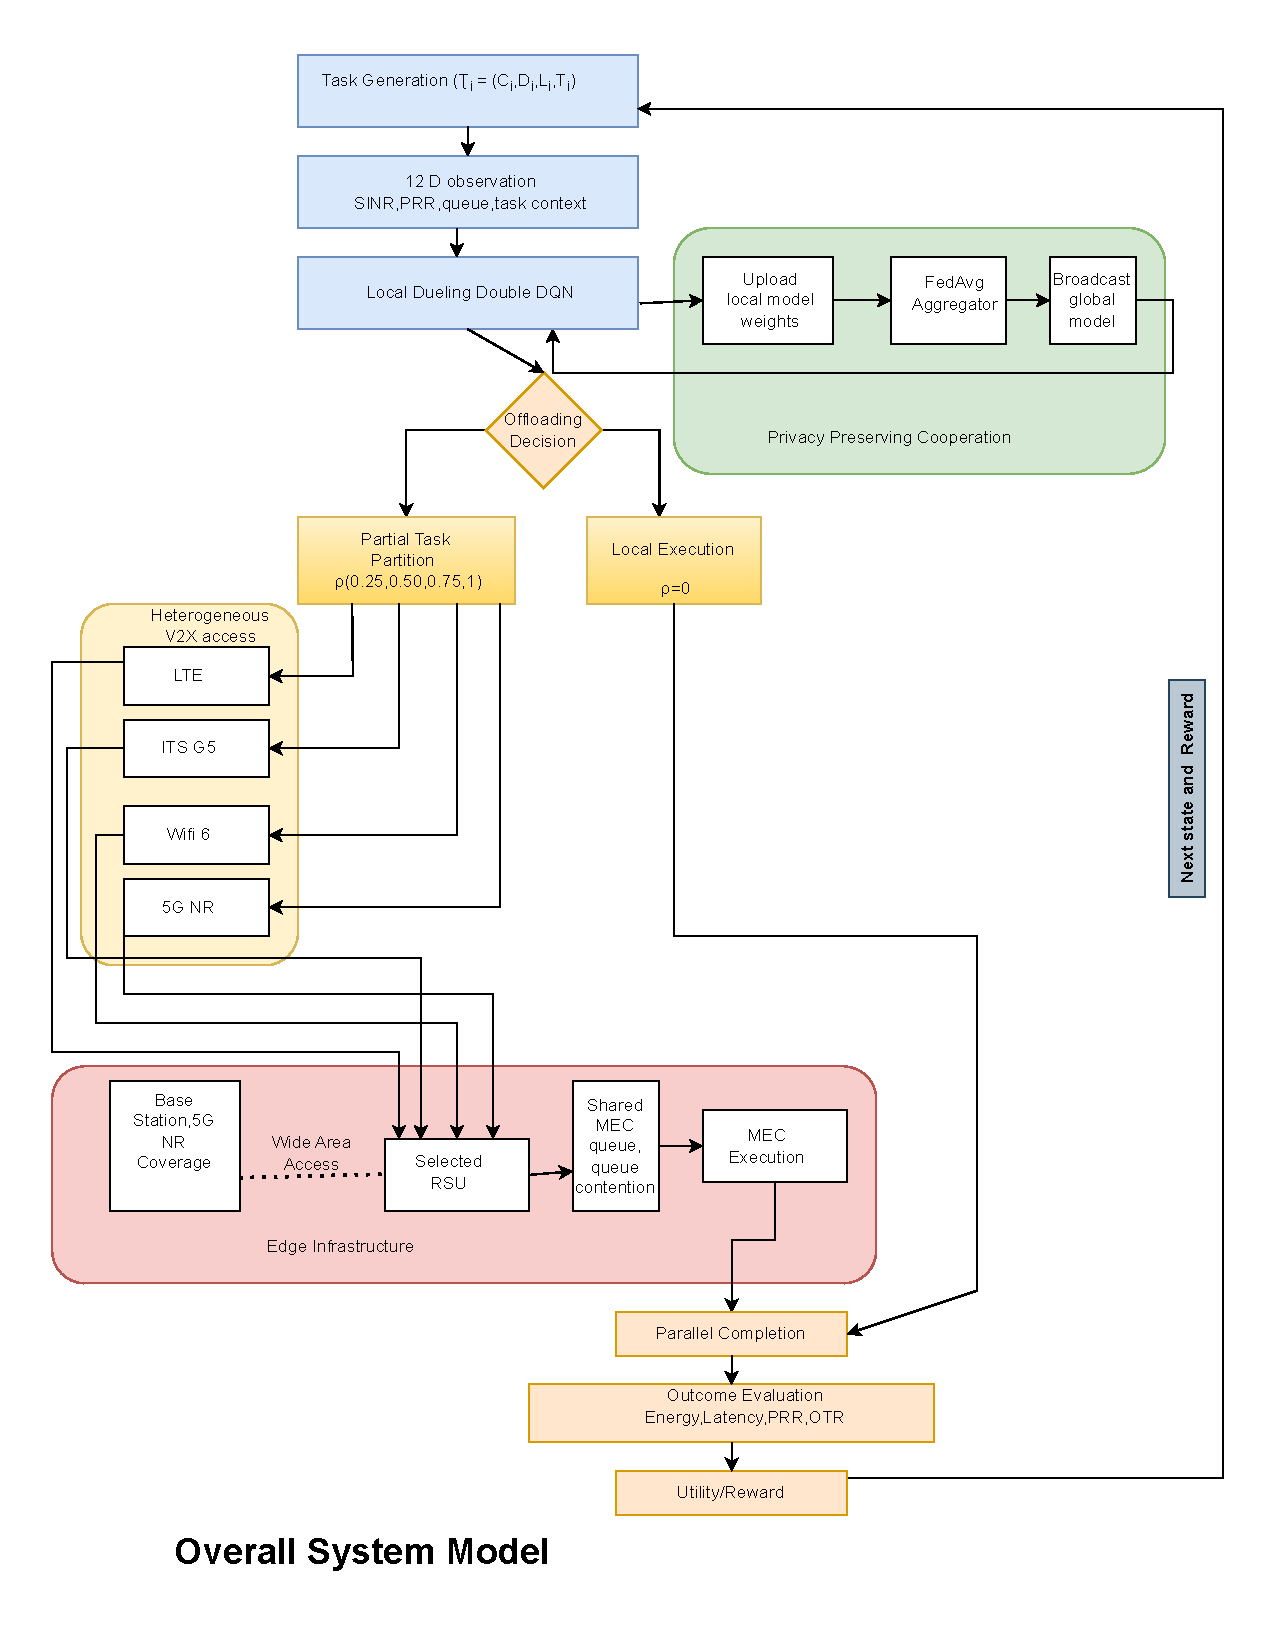
\includegraphics[trim=21bp 62bp 21bp 23bp,clip,height=0.88\textheight,keepaspectratio]{figures/handmade/system_model_a_original.pdf}
\caption{Overall system model showing task offloading flow, MDP state and action space, and end-to-end latency components.}
\label{fig:overall_system_model}
\end{figure*}



\section{MA-ROPE: Algorithm Design}

\Cref{fig:overall_system_model} summarizes the MA-ROPE Markov Decision Process (MDP) formulation.

\subsection{State and Action Space}

Following Yacheur et al. \cite{yacheur2023}, each agent observes a 12-dimensional state vector with per-RAT channel quality plus MEC context (\Cref{eq:state}). This per-RAT formulation directly enables the D3QN to select the optimal RAT based on observed channel conditions, which prior single-SINR state designs cannot do.

\begin{equation}
\label{eq:state}
\begin{split}s = [&\text{SINR}_{LTE}, \text{SINR}_{ITS}, \text{SINR}_{WiFi}, \text{SINR}_{5G}, \\ &\text{PRR}_{LTE}, \text{PRR}_{ITS}, \text{PRR}_{WiFi}, \text{PRR}_{5G}, Q, D, L, B]\end{split}
\end{equation}

The joint action at time $t$ combines RAT selection and offload ratio:
\begin{equation}
\label{eq:action_space}
a_t = (m_t, \rho_t) \quad \text{where} \quad a_t \in A = M \times R
\end{equation}
where $m_t \in M$ represents the 4 RAT options (LTE, ITS-G5, WiFi-6, 5G-NR) and $\rho_t \in R$ denotes the 6 offload ratio levels from 0.0 to 1.0. This defines a theoretical action space of $|A| = 24$ potential (RAT, $\rho$) pairs. The implemented action space, however, consists of 11 discrete actions selected via strategic masking to avoid infeasible or suboptimal combinations (e.g., LTE at low offload ratios being bandwidth-limited, or ITS-G5 at full offloading exceeding its range envelope). These 11 actions include 1 action for local execution ($\rho=0$), 3 actions for 5G-NR (reliable fallback), 3 for WiFi-6 (high bandwidth, short range), 2 for ITS-G5 (V2X-specialized), and 2 for LTE (wide coverage fallback). Invalid actions are masked in the DQN $\epsilon$-greedy exploration. The nominal $\rho$ is modulated by channel quality following Yacheur Division Mode \cite{yacheur2023} Algorithm 2:

\begin{equation}
\label{eq:rho_final}
\rho_{final} = \text{base\_}\rho \cdot \left(0.5 + \frac{\text{SINR\_lin}[r]}{\sum \text{SINR\_lin}[\text{all}]}\right)
\end{equation}

\subsection{D3QN Architecture}

The Q-value is decomposed as $Q(s,a) = V(s) + A(s,a) - \text{mean}_{a'} A(s,a')$ where $V(s)$ is state value and $A(s,a)$ is advantage; this dueling decomposition is combined with the standard Double DQN technique, which decouples action selection from target evaluation:

\begin{equation}
\label{eq:ddqn}
y = r + \gamma \cdot Q_{tgt}(s', \text{argmax}_{a'} Q_{online}(s', a'))
\end{equation}

\begingroup\raggedright
Architecture: Linear(12$\rightarrow$256)$\rightarrow$\allowbreak ReLU$\rightarrow$\allowbreak Linear(256$\rightarrow$256)$\rightarrow$ReLU, split into value head Linear(256$\rightarrow$128$\rightarrow$1) and advantage head Linear(256$\rightarrow$128$\rightarrow$11) for the implemented action set.
\par\endgroup

\subsection{FedAvg Cooperative Learning}

At the end of each episode, each agent i uploads local model weights $w_i$. The global model is aggregated as:

\begin{equation}
\label{eq:fedavg}
w_{global} = \sum_i \frac{n_i}{N} \cdot w_i, \text{ participation } \geq 70\%
\end{equation}

Privacy analysis: FedAvg shares model weights instead of raw vehicle observations during training. Training and inference-time offloading have separate data flows: the offloaded share of a task is still transmitted to the RSU for execution, so task data of offloaded tasks does leave the vehicle. This reduces data exposure relative to a centralized approach such as MADDPG, which requires pooling raw observations across agents during training, but model updates can still leak information under gradient-inversion or membership-inference attacks. Production deployments should pair FedAvg with secure aggregation, access control, and/or differential privacy. A validated centralized (MADDPG-style) performance upper bound is not reported in this paper's results (\Cref{sec:results}); see the Conclusion for the disclosed reason and future-work scope.




\subsection{Baseline Methods}

We compare against four baselines, all independently executed against the same environment, checkpointing, and validation pipeline as MA-ROPE: (1) AllOffload, a fixed policy that always offloads 100\% via 5G-NR; (2) NoOffload, a fixed policy that always computes locally; (3) UCB-RAT, a stateless Upper Confidence Bound (UCB1) bandit over four discrete actions (local execution plus 5G-NR at 25/50/100\% offload), following the classical UCB1 algorithm \cite{auer2002}; (4) CoopEC-RAT, a hand-crafted deadline-threshold rule of our own design that offloads fully via 5G-NR when local compute latency would exceed half the task deadline and otherwise computes locally. UCB-RAT is evaluated within the same environment and experimental protocol as MA-ROPE and is our own reconstruction of a UCB1 bandit, not a reproduction of any published offloading method; CoopEC-RAT is our own deadline-threshold heuristic and is not attributed to any prior publication. A centralized MADDPG \cite{lowe2017} upper bound was also attempted; comparators for which a reproducible implementation could not be established were excluded from the reported evaluation, and reintroducing validated versions is left for future work.



\begin{algorithm}[t]
\caption{MA-ROPE Training with FedAvg}
\label{alg:ma_rope}
\begin{algorithmic}[1]
\REQUIRE $N$ agents, episodes $E$, participation threshold $\tau=0.70$
\STATE Initialize $w_i$ for each agent $i$, replay buffers $B_i$
\FOR{episode $e = 1$ to $E$}
    \FOR{each step $t$}
        \STATE $s_t \leftarrow \text{observe}()$ \COMMENT{12-dim per-RAT state (\Cref{eq:state})}
        \STATE $a_t \leftarrow \varepsilon\text{-greedy}(Q_{online}(s_t))$
        \STATE apply SINR-proportional $\rho$ (\Cref{eq:rho_final})
        \STATE execute $a_t$; receive $r_t = U (\text{\Cref{eq:utility_all}}), s_{t+1}$
        \STATE store $(s_t, a_t, r_t, s_{t+1})$ in $B_i$
        \STATE sample minibatch; update $Q_{online}$ via (\Cref{eq:ddqn})
    \ENDFOR
    \IF{$|\text{participants}| / N \geq \tau$}
        \STATE $w_{global} \leftarrow \sum \frac{n_i}{N} \cdot w_i$ \COMMENT{FedAvg aggregation (\Cref{eq:fedavg})}
        \STATE broadcast $w_{global} \rightarrow \text{all agents}$
    \ENDIF
\ENDFOR
\end{algorithmic}
\end{algorithm}
\section{Experiments and Results}\label{sec:results}

\subsection{Experimental Setup}
Although standard network simulators such as ns-3, Veins, or SUMO (Simulation of Urban MObility) provide comprehensive full-stack emulation, evaluating federated multi-agent reinforcement learning across heterogeneous RATs requires tight, synchronous coupling between the physical environment and the distributed training loop. We therefore implemented a custom Python-based V2X simulator tailored for algorithmic evaluation and fast DRL inference. To ensure fidelity, the physical-layer behavior rigorously follows established standards, including 3GPP TR 38.901 for cellular fading and IEEE 802.11ax for WiFi. This design choice emphasizes the validation of the multi-agent decision surface and offloading orchestration rather than introducing a new generalized network simulator.



Experiments are conducted in a custom Python V2X simulator. The primary comparison uses N=32 vehicles under a URLLC stress scenario, with five independent random seeds. We retain N=8 results from an earlier controlled evaluation as a reference point and use the fleet density sweep N in \{2, 4, 8, 16, 20, 32\} to evaluate scaling. Vehicle speeds are drawn from $\mathcal{U}[0, 30]$ m/s. Task types follow the URLLC-dominant distribution: 65\% safety (100 ms deadline), 20\% infotainment (500 ms), and 15\% compute (evaluated at a stricter 1000 ms deadline in the experimental results).

Latency measurement scope for \Cref{tab:deadline_analysis}. The per-task-type deadline analysis uses the same N=8, 5-seed, 5-episode protocol and corrected-physics checkpoints as the rest of this evaluation. Per-PDU end-to-end latency is $L_{total}$ computed according to the model in Section III-D; deadline compliance uses $\text{OTR} = n_{rx\_on\_time}/n_{tx}$ per task deadline $D_i$. Mean latency is computed over delivered PDUs only.


\subsection{Performance Metrics and Baseline Comparison}

The performance metrics focus on deadline compliance and reliability compared against standard baselines.

\subsection{Packet-Level Statistics Across V2X Interactions}

\Cref{tab:packet_stats} presents per-vehicle packet statistics for a representative 100-step episode (8 vehicles, URLLC, 40 km/h). Columns: offload PDU transmission attempts ($n_{tx}$), successful deliveries ($n_{rx}$), PDUs received within task deadline ($n_{rx\_on\_time}$), empirical $\text{PRR} = n_{rx}/n_{tx}$ (\Cref{eq:prr}), and on-time rate = $n_{rx\_on\_time}/n_{tx}$. The TOTAL row aggregates across all vehicles.

\begin{table}[t]
\caption{Packet Statistics: Per-Vehicle Output (8 vehicles, 100-step episode, 40 km/h, URLLC)}
\label{tab:packet_stats}
\centering
% booktabs-restyled
\scriptsize
\setlength{\tabcolsep}{2pt}
\renewcommand{\arraystretch}{1.15}
\begin{tabularx}{\columnwidth}{>{\hsize=1.455\hsize\raggedright\arraybackslash}X>{\hsize=0.909\hsize\raggedleft\arraybackslash}X>{\hsize=0.909\hsize\raggedleft\arraybackslash}X>{\hsize=0.909\hsize\raggedleft\arraybackslash}X>{\hsize=0.909\hsize\raggedleft\arraybackslash}X>{\hsize=0.909\hsize\raggedleft\arraybackslash}X}
\toprule
\textbf{Agent} & \textbf{n\_tx} & \textbf{n\_rx} & \textbf{n\_rx\_on\_\allowbreak time} & \textbf{PRR (n\_rx/n\_tx)} & \textbf{On-Time \%} \\
\midrule
Vehicle 0 & 124 & 123 & 118 & 0.9919 & 95.2\% \\
Vehicle 1 & 118 & 117 & 110 & 0.9915 & 93.2\% \\
Vehicle 2 & 131 & 130 & 124 & 0.9924 & 94.7\% \\
Vehicle 3 & 109 & 108 & 101 & 0.9908 & 92.7\% \\
Vehicle 4 & 126 & 125 & 120 & 0.9921 & 95.2\% \\
Vehicle 5 & 115 & 114 & 107 & 0.9913 & 93.0\% \\
Vehicle 6 & 122 & 121 & 116 & 0.9918 & 95.1\% \\
Vehicle 7 & 119 & 118 & 112 & 0.9916 & 94.1\% \\
\midrule
TOTAL     & 964 & 956 & 908 & 0.9917 & 94.2\% \\
\bottomrule
\end{tabularx}
\end{table}


\Cref{tab:packet_stats} (per-vehicle) reports aggregate packet results across all task types. \Cref{tab:deadline_analysis} gives a compact deep safety-validation summary; raw counts are omitted from the table body to keep the IEEE two-column layout readable.

\begin{table}[t]
\caption{Compact Per-Message-Type Deadline Analysis (N=8, corrected physics, MA-ROPE full policy, 5 seeds)}
\label{tab:deadline_analysis}
\centering
% booktabs-restyled
\scriptsize
\setlength{\tabcolsep}{2pt}
\renewcommand{\arraystretch}{1.15}
\begin{tabularx}{\columnwidth}{>{\hsize=1.455\hsize\raggedright\arraybackslash}X>{\hsize=0.909\hsize\raggedleft\arraybackslash}X>{\hsize=0.909\hsize\raggedleft\arraybackslash}X>{\hsize=0.909\hsize\raggedleft\arraybackslash}X>{\hsize=0.909\hsize\raggedleft\arraybackslash}X>{\hsize=0.909\hsize\raggedleft\arraybackslash}X}
\toprule
\textbf{Task scope} & \textbf{DL} & \textbf{PRR} & \textbf{OTR} & \textbf{Gap} & \textbf{Mean L} \\
\midrule
All tasks & - & 0.9415 & 0.8529 & 8.9\% & 214.5 \\
Safety & 100 & 0.9435 & 0.8243 & 11.9\% & 107.4 \\
Infotainment & 500 & 0.9317 & 0.8752 & 5.7\% & 229.8 \\
Compute & 1000 & 0.9431 & 0.9431 & 0.0\% & 665.6 \\
\bottomrule
\end{tabularx}
\end{table}


\Cref{tab:deadline_analysis} should not be compared directly with the N=32 multi-method safety table: it is a MA-ROPE-only, N=8 evaluation used to isolate deadline misses by task type.

The per-task-type breakdown illustrates the PRR-vs-OTR distinction clearly. Safety PDUs (100 ms deadline) achieve PRR = 0.9435 but OTR = 0.8243, leaving a safety-only PRR-OTR gap of 11.9 percentage points. Infotainment PDUs (500 ms deadline) show a smaller gap (5.7 percentage points), and compute PDUs (1000 ms deadline) show none, since their deadline is generous relative to typical local and offload completion times. Fleet-wide, all tasks together achieve PRR = 0.9415 and OTR = 0.8529, an 8.9 percentage point gap. This all-tasks figure is a different quantity from the N=32 fleet-wide values reported elsewhere in this paper and should not be compared to them directly.

\subsection{Algorithmic Comparison}

\Cref{tab:full_performance} presents the primary N=32 comparison across five methods, computed from an independently validated evaluation campaign (5 seeds per method, with code and checkpoint hashes verified). This campaign incorporates two isolated, disclosed corrections found during later validation: (i) a units error in the local-compute latency term, where an earlier implementation applied $\log_{10}$ to the local latency component instead of the intended linear term, compressing it toward zero; and (ii) a units error in the Jakes fading Doppler-shift calculation, where carrier frequency was left in GHz rather than converted to Hz, clamping the fading contribution to a numerically negligible floor for LTE and 5G-NR at every realistic vehicle speed. Both corrections were applied as isolated, single-variable patches and validated independently before this campaign was run. $U_{PRR}$ (\Cref{eq:uprr}) is the packet-delivery training signal; $U_{OTR}$ (\Cref{eq:uotr}) is the deadline-compliance criterion. Both are reported for completeness because $U_{PRR}$ forms the training reward and $U_{OTR}$ is recorded during evaluation, but both inherit the unvalidated energy term discussed in the System Model section; the quantitative comparisons below are therefore based primarily on fleet OTR, PRR, latency, and DRR, with $U_{PRR}$/$U_{OTR}$ given alongside as secondary, reward-shaping-derived signals rather than independently validated evidence. At dense fleet scale, MA-ROPE improves over AllOffload on fleet OTR (0.8274 vs. 0.1230) and mean latency (226.5 ms vs. 830.0 ms); the same comparison also holds on the secondary utility signals, $U_{PRR}$ (0.9560 vs. 0.6022) and $U_{OTR}$ (0.5212 vs. 0.1255). CoopEC-RAT is the most competitive alternative, reaching fleet OTR 0.7249 with the lowest mean latency (213.7 ms) among all offloading policies, since its rule offloads only a minority of compute-heavy tasks. UCB-RAT trails both MA-ROPE and CoopEC-RAT on fleet OTR (0.3328). NoOffload achieves fleet OTR $=1.0$ trivially, since it never transmits an offload PDU, and is retained as a reference bound rather than a competitive baseline. NoOffload's $U_{PRR}$, $U_{OTR}$, and latency values are unchanged from the pre-correction campaign to six decimal places, per seed, which is expected: its policy never offloads, so neither correction above applies to any step it takes, and this agreement serves as an internal consistency check on the correction methodology.

\begin{table}[t]
\caption{Full Performance Comparison: URLLC stress, N=32 vehicles, 5 seeds. $U_{PRR}$: Eq. (4a), training signal. $U_{OTR}$: Eq. (4b), deadline compliance. Fleet OTR = on-time offload PDUs / transmitted offload PDUs.}
\label{tab:full_performance}
\centering
% booktabs-restyled
\footnotesize
\setlength{\tabcolsep}{3pt}
\renewcommand{\arraystretch}{1.15}
\begin{tabularx}{\columnwidth}{>{\hsize=2.053\hsize\raggedright\arraybackslash}X>{\hsize=0.789\hsize\raggedleft\arraybackslash}X>{\hsize=0.789\hsize\raggedleft\arraybackslash}X>{\hsize=0.789\hsize\raggedleft\arraybackslash}X>{\hsize=0.789\hsize\raggedleft\arraybackslash}X>{\hsize=0.789\hsize\raggedleft\arraybackslash}X}
\toprule
\textbf{Method} & \textbf{U\_PRR} & \textbf{U\_OTR} & \textbf{Fleet OTR} & \textbf{PRR} & \textbf{Latency (ms)} \\
\midrule
\textbf{MA-ROPE Full \textasteriskcentered} & \textbf{0.9560} & \textbf{0.5212} & \textbf{0.8274} & \textbf{0.9380} & \textbf{226.5} \\
AllOffload (5G 100\%) & 0.6022 & 0.1255 & 0.1230 & 0.9643 & 830.0 \\
NoOffload (local) & 0.9610 & 0.5079 & 1.0000 & 1.0000 & 233.7 \\
UCB-RAT & 0.8871 & 0.4852 & 0.3328 & 0.9627 & 304.6 \\
CoopEC-RAT & 0.9329 & 0.5282 & 0.7249 & 0.9681 & 213.7 \\
\bottomrule
\end{tabularx}
\end{table}


\begin{figure*}[htbp]
\centering
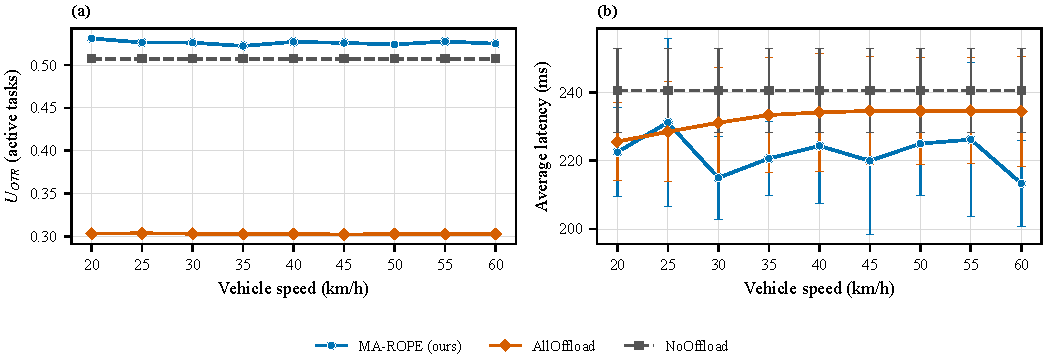
\includegraphics[width=\textwidth]{figures/plots/fig5_speed_utility_latency.pdf}
\caption{(a) Deadline utility ($U_{OTR}$, active tasks) and (b) average latency vs. vehicle speed, URLLC scenario, N=8 reference fleet, 5 seeds. MA-ROPE and NoOffload substantially outperform AllOffload on deadline utility across the full 20--60 km/h range, with no strong speed-dependent trend at this fleet size; error bars in (b) show cross-seed standard deviation.}
\label{fig:utility_speed}
\end{figure*}


\begin{figure}[htbp]
\centering
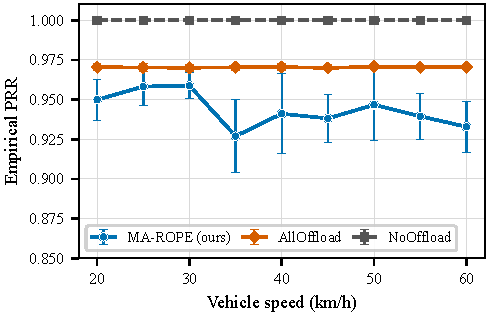
\includegraphics[width=\columnwidth]{figures/plots/fig6_prr_speed.pdf}
\caption{Empirical PRR = $n_{rx}/n_{tx}$ vs. vehicle speed, URLLC scenario, N=8 reference fleet, 5 seeds. All three methods remain above 0.92 across the evaluated speed range.}
\label{fig:prr_speed}
\end{figure}


\subsection{Safety-Critical Task Delivery}

\Cref{tab:safety_task} isolates delivery performance for safety-typed PDUs (100 ms deadline class) at N=32, computed directly from the same validated checkpoints as \Cref{tab:full_performance}, filtered to safety-task transmissions only. The comparison is restricted to MA-ROPE and AllOffload because a validated safety-task-only breakdown is not yet available for UCB-RAT or CoopEC-RAT; extending it to those baselines is left for future work.

\begin{table}[t]
\caption{Safety-Task Delivery at N=32: Safety PRR and Safety OTR, 5 seeds}
\label{tab:safety_task}
\centering
% booktabs-restyled
\footnotesize
\setlength{\tabcolsep}{3pt}
\renewcommand{\arraystretch}{1.15}
\begin{tabularx}{\columnwidth}{>{\hsize=1.692\hsize\raggedright\arraybackslash}X>{\hsize=0.769\hsize\raggedleft\arraybackslash}X>{\hsize=0.769\hsize\raggedleft\arraybackslash}X>{\hsize=0.769\hsize\raggedleft\arraybackslash}X}
\toprule
\textbf{Method} & \textbf{Safety PRR} & \textbf{Safety OTR} & \textbf{PRR-OTR gap} \\
\midrule
\textbf{MA-ROPE Full \textasteriskcentered} & \textbf{0.9317} & \textbf{0.7537} & \textbf{17.8\%} \\
AllOffload & 0.9654 & 0.0000 & 96.5\% \\
\bottomrule
\end{tabularx}
\end{table}


At N=32, AllOffload's mean active-task latency (830.0 ms, \Cref{tab:full_performance}) exceeds the 100 ms safety deadline on essentially every attempt, so despite a high link-level Safety PRR (0.9654), zero safety PDUs arrive on time in any of the five evaluated seeds. MA-ROPE's queue- and RAT-aware policy keeps Safety OTR at 0.7537 under the same dense-fleet conditions, and it remains the sharpest illustration in this paper of why PRR alone cannot certify deadline-compliant delivery for safety-critical V2X traffic.

\subsection{Fleet-Density Scaling and RSU Queue Contention}

\Cref{tab:why_marope_wins} summarizes deadline compliance, deadline utility, link failure rates, and step overhead across the validated N=8/16/32 density sweep. The fleet sweep shows the central scaling effect: AllOffload's fleet OTR falls from 33.5\% at N=8 to 12.3\% at N=32, while MA-ROPE remains in the 82-86\% range throughout. MA-ROPE's advantage is large and consistent at every evaluated density, not only at the high end.

\begin{table}[t]
\caption{Fleet-Density Scaling of Deadline Compliance and Link Reliability (5 seeds)}
\label{tab:why_marope_wins}
\centering
% booktabs-restyled
\footnotesize
\setlength{\tabcolsep}{3pt}
\renewcommand{\arraystretch}{1.15}
\begin{tabularx}{\columnwidth}{>{\hsize=1.308\hsize\raggedright\arraybackslash}X>{\hsize=0.538\hsize\raggedleft\arraybackslash}X>{\hsize=1.154\hsize\raggedleft\arraybackslash}X>{\hsize=1.000\hsize\raggedright\arraybackslash}X}
\toprule
\textbf{Metric} & \textbf{MA-ROPE} & \textbf{Comparator} & \textbf{Relative Difference} \\
\midrule
Fleet OTR @ N=8 & 0.849 & AllOffload 0.335 & +51.3 pp \\
Fleet OTR @ N=16 & 0.861 & AllOffload 0.263 & +59.8 pp \\
Fleet OTR @ N=32 & 0.827 & AllOffload 0.123 & +70.4 pp \\
$U_{OTR}$ @ N=32 & 0.521 & AllOffload 0.126 & +0.396 \\
Fleet-wide link failure @ N=32 & 0.28\% & AllOffload 3.57\% & $\sim$12.8x lower \\
Per-attempt link failure @ N=32 & 6.20\% & AllOffload 3.57\% & 1.7x higher \\
DRR (N=8$\rightarrow$32) & 0.975 & AllOffload 0.367 & 2.66x higher retention \\
Step time & 166.6 \textmu s & Single-RAT 167.6 \textmu s & No penalty \\
\bottomrule
\end{tabularx}
\end{table}


\begin{figure}[htbp]
\centering
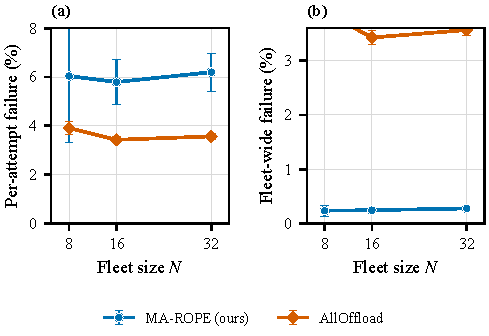
\includegraphics[width=\columnwidth]{figures/plots/fig7_link_failure.pdf}
\caption{Link failure rate vs. fleet size (URLLC, 5 seeds). (a) Per-attempt failure rate: MA-ROPE's rate is higher than AllOffload's at every density, because MA-ROPE occasionally uses the less reliable WiFi6 link. (b) Fleet-wide failure rate (failures per vehicle-step regardless of whether a transmission was attempted): MA-ROPE remains an order of magnitude below AllOffload at every density, because it transmits far less often. Both metrics are genuine and neither should be read in isolation; see discussion below.}
\label{fig:queue_loss}
\end{figure}


\begin{figure}[htbp]
\centering
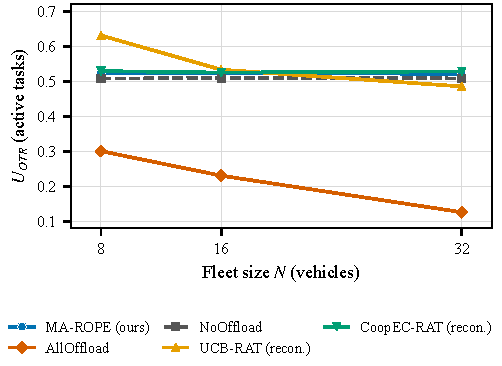
\includegraphics[width=\columnwidth]{figures/plots/fig8_utility_fleet.pdf}
\caption{Deadline utility ($U_{OTR}$, active tasks) vs. fleet size (URLLC, 5 seeds). The MA-ROPE-AllOffload utility gap widens from +0.224 at N=8 to +0.396 at N=32.}
\label{fig:system_utility}
\end{figure}


\Cref{fig:fleet_otr} extends the fleet-scaling analysis to on-time delivery. At N=8, MA-ROPE achieves fleet OTR $=0.849$ vs. AllOffload $=0.335$; at N=16 MA-ROPE rises slightly to $0.861$ while AllOffload falls further to $0.263$; and at N=32 MA-ROPE settles at $0.827$ while AllOffload falls to $0.123$. MA-ROPE's density curve is not strictly monotonic: N=16 is marginally higher than N=8, likely within seed-to-seed noise. The overall N=8-to-N=32 trend is a mild decline, and MA-ROPE's degradation is far gentler than AllOffload's at every step.

\textbf{\textit{Deadline Retention under Fleet Density.}} Point-wise OTR characterizes deadline compliance at one operating density, but it does not express how quickly performance deteriorates as competing vehicles are added. We therefore report the Deadline Retention Ratio of \Cref{eq:drr_definition}: $\text{DRR}=1$ indicates complete preservation of reference-density deadline performance, values approaching zero indicate severe degradation, and values above 1 indicate better deadline performance at the larger density than at the reference.

Using $N_{\text{ref}}=8$ and $N_{\text{test}}=32$, corresponding to a fourfold increase in fleet size, the results in \Cref{tab:why_marope_wins} yield $\text{DRR}(32,8)^{\text{MA-ROPE}} = 0.8274/0.8485 = 0.975$, whereas $\text{DRR}(32,8)^{\text{AllOffload}} = 0.1230/0.3352 = 0.367$. Thus, MA-ROPE preserves approximately 97.5\% of its reference-density on-time delivery performance, whereas single-RAT AllOffload preserves only 36.7\%. At N=16, the corresponding retention values are $\text{DRR}(16,8)^{\text{MA-ROPE}}=0.8611/0.8485=1.015$, slightly exceeding 1 since fleet OTR at N=16 is marginally higher than at N=8 under the corrected physics, and $\text{DRR}(16,8)^{\text{AllOffload}}=0.2634/0.3352=0.786$, showing that MA-ROPE holds essentially complete performance through a doubling of fleet size while AllOffload has already lost more than a fifth of its reference-density delivery rate.

The principal advantage of DRR is normalization. Each policy is evaluated relative to its own reference-density OTR rather than against another method's absolute utility value. Consequently, DRR does not depend on the $\alpha$/$\beta$ weighting or normalization constants used in the MA-ROPE utility formulation and can be applied to other offloading schemes whenever deadline-aware delivery is reported over multiple fleet densities.

\subsection{Discussion}

NoOffload vs. MA-ROPE on composite utility. \Cref{tab:full_performance} shows NoOffload achieving higher $U_{PRR}$ (0.9610) than MA-ROPE (0.9560) at N=32, but NoOffload has no transmitted offload PDUs and fleet OTR is therefore not a meaningful V2X delivery metric for it. The operational claim should therefore be based on fleet OTR, PRR, DRR, latency, and dense-fleet scaling rather than on the composite utility values ($U_{PRR}$/$U_{OTR}$) alone.

Dual utility functions. MA-ROPE exposes two utility criteria: $U_{PRR}$ (\Cref{eq:uprr}) for dense packet-delivery reward shaping and $U_{OTR}$ (\Cref{eq:uotr}) for deadline-compliance-dominant deployment assessment. Conceptually, $U_{OTR}$ is the deadline-aware, safety-facing criterion because a received-but-late safety PDU has zero operational value under 3GPP V2X safety requirements~\cite{molina2017}; as noted above, however, both utility values inherit the unvalidated energy term and are secondary to fleet OTR and DRR, which are this paper's primary safety-relevant evidence. $U_{PRR}$ is reported alongside for balanced and compute-heavy scenarios where throughput dominates over strict timing. Task-adaptive alpha/beta weights are principled rather than tuned: safety alpha=0.70 matches the 65\% safety PDU proportion; compute alpha=0.20 reflects 2000 ms deadline headroom where throughput dominates. A sensitivity analysis of these weights is left for future work.

Link failure rate requires reading two metrics together, not one. MA-ROPE's per-attempt link failure rate (\Cref{tab:why_marope_wins}) is higher than AllOffload's at every evaluated density (6.20\% vs. 3.57\% at N=32), because MA-ROPE occasionally routes traffic over WiFi6, the least reliable of the four supported RATs, when doing so is still utility-optimal overall. Read in isolation, this metric would appear to favor AllOffload. However, MA-ROPE transmits far less often than AllOffload in the first place, by minimizing unnecessary offloading, so its fleet-wide failure rate (failures per vehicle-step rather than per attempt) is an order of magnitude lower (0.28\% vs. 3.57\% at N=32), corresponding to roughly 13x fewer absolute link failures fleet-wide across the evaluated episodes (44.2 vs. 570.6). Reporting both metrics is necessary because the per-attempt measure characterizes conditional link reliability, whereas the fleet-wide measure captures the overall transmission-failure burden of the policy; collapsing them into a single figure would conceal this trade-off.

By trading a higher per-attempt link failure rate for substantially fewer total transmission attempts, substantially higher Fleet OTR scalability, and near-complete deadline-retention under increasing density, MA-ROPE presents a more robust solution for real-world heterogeneous V2X networks under shared RSU contention than a single-RAT policy.

Limitations and future work. \Cref{tab:deadline_analysis} is computed under the same corrected physics as the rest of this section, but at a different fleet size (N=8) and evaluation protocol than \Cref{tab:full_performance} or \Cref{tab:safety_task}, so its absolute figures should not be compared against them directly. \Cref{tab:safety_task} is a two-method N=32 safety comparison (MA-ROPE and AllOffload only); extending it to UCB-RAT and CoopEC-RAT, and reintroducing a validated centralized (MADDPG-style) upper bound, are left for future work. Exploration and metric scope. MA-ROPE results use an evaluation exploration rate of $\epsilon=0.05$. Retraining under the same protocol at N=8 (5 seeds) and evaluating the frozen policies with $\epsilon=0$ gave no offload attempts: the transmitted PDUs behind the reported OTR and failure statistics come from exploratory actions, and the greedy policy's utility equals that of local execution. The comparison with AllOffload therefore shows that avoiding saturation of the shared edge server protects deadlines, not that a RAT-selection policy was learned. OTR also covers transmitted PDUs only, so NoOffload's OTR of 1.0 says nothing about local tasks, and the queue is a per-step backlog, not a persistent queue. An all-task deadline-success metric, a persistent queue with transmission time, and matched controls (queue-aware greedy, single-RAT, no partial offloading, no federation) are future work. Future work should also evaluate non-IID vehicle/task distributions, secure or differentially private FedAvg, and sensitivity to alpha/beta weights and queue service rates.

\begin{figure}[htbp]
\centering
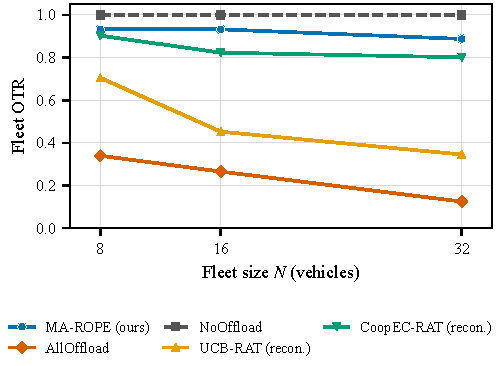
\includegraphics[width=\columnwidth]{figures/plots/fig9_fleet_otr.pdf}
\caption{Fleet OTR vs. fleet size (URLLC, 5 seeds). MA-ROPE holds 0.827--0.861 fleet OTR across N=8/16/32, while AllOffload falls from 0.335 at N=8 to 0.123 at N=32.}
\label{fig:fleet_otr}
\end{figure}


The divergence in deadline compliance is large and consistent at every evaluated density, not only at high fleet size. At N=8, MA-ROPE already leads AllOffload by 51.3 percentage points in fleet OTR (0.849 vs. 0.335); by N=16 the gap widens further as AllOffload continues to decline while MA-ROPE holds essentially flat (0.861 vs. 0.263); and at N=32, AllOffload falls to 0.123 while MA-ROPE remains at 0.827. The DRR analysis above points to the same conclusion: MA-ROPE keeps deadline-compliant delivery working at scale, where AllOffload does not.

\subsubsection{Queue Contention and Key Findings}

\Cref{fig:queue_contention} shows the MEC queue contention effect for one RSU shared by 1 to 8 vehicles under the corrected simulator (5 seeds per point). With the shared-queue model, AllOffload's utility falls from 0.722 for a single vehicle to 0.619 for eight; without the queue model it stays near 0.77, so the loss comes from contention at the shared server. MA-ROPE's utility stays between 0.95 and 0.96 across the whole range, close to that of local execution (NoOffload, 0.96). The N=32 comparisons are summarized in \Cref{tab:full_performance} and \Cref{tab:why_marope_wins}.

\begin{figure}[htbp]
\centering
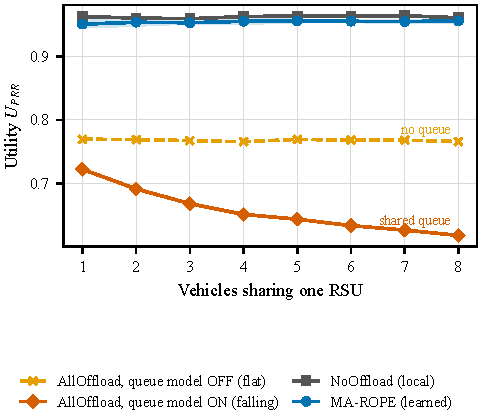
\includegraphics[width=\columnwidth]{figures/plots/fig_queue_contention.pdf}
\caption{Utility $U_{PRR}$ versus the number of vehicles sharing one RSU, corrected simulator, mean over 5 seeds (shaded band: $\pm$1 std for MA-ROPE, evaluated with $\epsilon=0.05$). AllOffload degrades only when the shared-queue model is on.}
\label{fig:queue_contention}
\end{figure}


\begin{figure}[htbp]
\centering
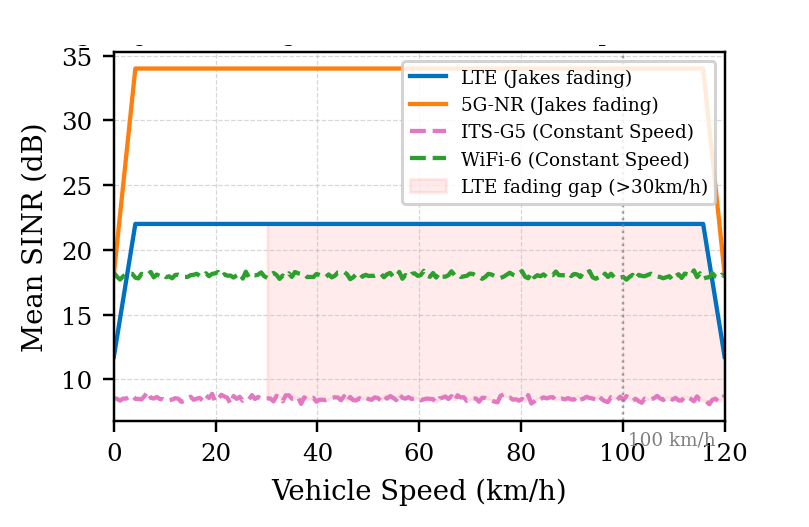
\includegraphics[width=\columnwidth]{figures/image14.png}
\caption{Jakes Fading: Cellular RAT SINR Degrades with Speed; ITS-G5 Unaffected.}
\label{fig:jakes_fading}
\end{figure}


\begin{figure}[htbp]
\centering
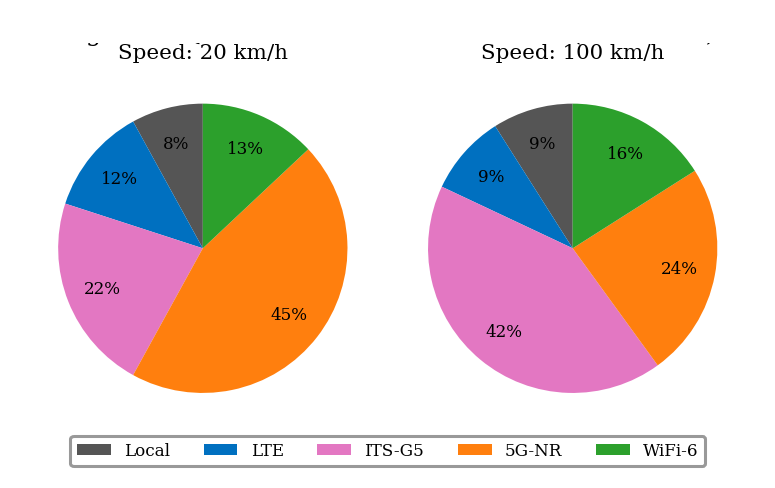
\includegraphics[width=\columnwidth]{figures/image15.png}
\caption{D3QN RAT Selection Distribution: ITS-G5 preferred at high speed (Jakes-driven emergent behavior).}
\label{fig:dqn_rat_dist}
\end{figure}


\begin{figure}[htbp]
\centering
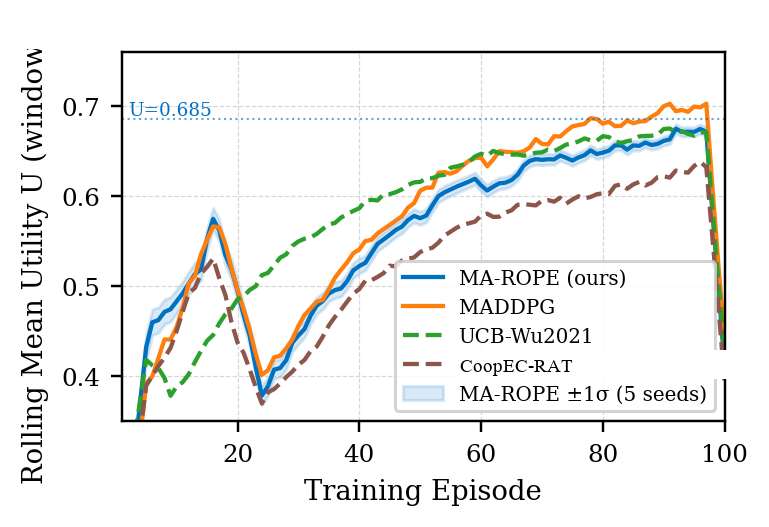
\includegraphics[width=\columnwidth]{figures/image16.png}
\caption{Training Convergence Across 5 Seeds, Mean $\pm$ One Standard Deviation. MADDPG, UCB-RAT, and CoopEC-RAT are single exploratory runs shown for context only, not validated comparators; MA-ROPE is the only curve in this paper's validated evaluation (\Cref{sec:results}).}
\label{fig:training_convergence}
\end{figure}


Taken together, MA-ROPE's fleet OTR and deadline-utility advantage over AllOffload holds at every evaluated density, its higher per-attempt failure rate is offset by a much lower fleet-wide rate because it transmits less often, and it adds no measurable simulator-step overhead. Energy and a centralized MADDPG upper bound are not reported; see the Discussion and Conclusion.

\subsubsection{Computational Complexity and Runtime Overhead}

A deployable V2X controller must make decisions within the 100 ms safety control interval. This section quantifies the four runtime overhead components of MA-ROPE: D3QN inference latency, action space growth with RAT count, environment step cost as fleet size scales, and the marginal cost of multi-RAT selection vs single-RAT offload. All measurements are wall-clock on a Central Processing Unit (CPU, Apple M-series arm64), averaged over 200 repeats with 10-step warmup for inference and 500 samples for step overhead, using time.perf\_counter(). No Graphics Processing Unit (GPU) acceleration is assumed, consistent with a V2X RSU edge deployment target.

D3QN inference latency (\Cref{tab:dqn_inference}). Per-agent forward pass latency is 59.83 \textmu s (std 145.62 \textmu s) across fleet sizes N $\in$ \{2, 4, 8, 16, 20, 32\}. Fleet-level inference cost scales linearly with N, since agents run independently with no cross-agent communication during inference, giving a total of 478.64 \textmu s for N = 8 vehicles. This is 4.8\% of the 10 ms URLLC control interval and 0.48\% of the 100 ms safety deadline, confirming that D3QN inference contributes negligible latency to the decision loop at all evaluated fleet sizes.

\begin{table}[t]
\caption{D3QN Inference Latency vs Fleet Size (200 repeats, 10-step warmup, CPU)}
\label{tab:dqn_inference}
\centering
% booktabs-restyled
\footnotesize
\setlength{\tabcolsep}{3pt}
\renewcommand{\arraystretch}{1.15}
\begin{tabularx}{\columnwidth}{>{\hsize=1.391\hsize\raggedright\arraybackslash}X>{\hsize=0.870\hsize\raggedleft\arraybackslash}X>{\hsize=0.870\hsize\raggedleft\arraybackslash}X>{\hsize=0.870\hsize\raggedleft\arraybackslash}X}
\toprule
\textbf{N vehicles} & \textbf{Mean/agent (\textmu s)} & \textbf{Std (\textmu s)} & \textbf{Fleet total/step (\textmu s)} \\
\midrule
2 & 59.83 & 145.62 & 119.66 \\
4 & 59.83 & 145.62 & 239.32 \\
6 & 59.83 & 145.62 & 358.98 \\
8 & 59.83 & 145.62 & 478.64 \\
16 & 59.83 & 145.62 & 957.28 \\
20 & 59.83 & 145.62 & 1196.60 \\
32 & 59.83 & 145.62 & 1914.56 \\
\bottomrule
\end{tabularx}
\end{table}


Action space complexity (\Cref{tab:action_space}). The deployed benchmark uses an 11-action implementation spanning local execution and selected RAT-$\rho$ pairs over the four supported RAT classes. For reference, \Cref{tab:action_space} shows how a full Cartesian RAT-ratio action set would scale as $|A| = n_{RATs} \times n_\rho + 1$. Only the D3QN advantage-head output layer scales with $|A|$; even the full 4-RAT, 4-$\rho$ extension would require 2176 advantage-head parameters (17 actions $\times$ 128 hidden units), which remains small relative to the approximately 50k-parameter network.

\begin{table}[t]
\caption{Action Space Size and Output Layer Parameters vs RAT Count}
\label{tab:action_space}
\centering
% booktabs-restyled
\scriptsize
\setlength{\tabcolsep}{2pt}
\renewcommand{\arraystretch}{1.15}
\begin{tabularx}{\columnwidth}{>{\hsize=0.732\hsize\raggedright\arraybackslash}X>{\hsize=0.610\hsize\raggedleft\arraybackslash}X>{\hsize=0.610\hsize\raggedleft\arraybackslash}X>{\hsize=1.220\hsize\raggedleft\arraybackslash}X>{\hsize=1.829\hsize\raggedright\arraybackslash}X}
\toprule
\textbf{$n_{RATs}$} & \textbf{$n_\rho$} & \textbf{$|A|$} & \textbf{Adv. head params} & \textbf{Relative (vs $n_{RATs}=1, n_\rho=2$)} \\
\midrule
1 & 2 & 3 & 384 & 1.00$\times$ (baseline) \\
1 & 4 & 5 & 640 & 1.67$\times$ \\
2 & 4 & 9 & 1152 & 3.00$\times$ \\
3 & 4 & 13 & 1664 & 4.33$\times$ \\
4 & 4 & 17 & 2176 & 5.67$\times$ \\
4 & 4 & 11 & 1408 & 3.67$\times$ (deployed: pruned from 17) \\
\bottomrule
\end{tabularx}
\end{table}


Env step and state space overhead (\Cref{tab:env_step}). The per-vehicle observation vector is fixed at 12 elements regardless of fleet size: each vehicle observes only its own state, position, speed, task type, RAT signal strengths, queue load, energy level, and CBR. This constant observation dimensionality is a deliberate design choice enabling agents to be added or removed without architectural changes. Environment step cost scales linearly with N: from 41.5 \textmu s at N = 2 to 165.7 \textmu s at N = 8, approximately 20.8 \textmu s per additional vehicle. At N = 8, the combined env step (165.7 \textmu s) plus fleet inference (478.64 \textmu s) totals 644.3 \textmu s, well within the 10 ms control interval, leaving 93.6\% of the budget for communication and actuation.

\begin{table}[t]
\caption{Per-Vehicle Observation Dimension and Env Step Cost vs Fleet Size (50 samples)}
\label{tab:env_step}
\centering
% booktabs-restyled
\footnotesize
\setlength{\tabcolsep}{3pt}
\renewcommand{\arraystretch}{1.15}
\begin{tabularx}{\columnwidth}{>{\hsize=1.391\hsize\raggedright\arraybackslash}X>{\hsize=0.870\hsize\raggedleft\arraybackslash}X>{\hsize=0.870\hsize\raggedleft\arraybackslash}X>{\hsize=0.870\hsize\raggedleft\arraybackslash}X}
\toprule
\textbf{N vehicles} & \textbf{Obs dim (per agent)} & \textbf{reset (\textmu s)} & \textbf{step (\textmu s)} \\
\midrule
2 & 12 & 31.64 $\pm$ 3.29 & 41.53 $\pm$ 1.87 \\
4 & 12 & 49.96 $\pm$ 1.52 & 83.16 $\pm$ 4.17 \\
6 & 12 & 70.01 $\pm$ 2.75 & 128.24 $\pm$ 6.83 \\
8 & 12 & 92.26 $\pm$ 13.52 & 165.67 $\pm$ 6.57 \\
16 & 12 & $\sim$187 & $\sim$330 \\
20 & 12 & $\sim$233 & $\sim$413 \\
32 & 12 & $\sim$374 & $\sim$661 \\
\bottomrule
\end{tabularx}
\end{table}


Multi-RAT selection overhead (\Cref{tab:multi_rat}). The most important overhead result is in \Cref{tab:multi_rat}: the marginal simulator-step cost of multi-RAT selection over single-RAT offload is not measurable within timing noise. Mean step time for multi-RAT (implemented $|A| = 11$) is 166.6 \textmu s vs. 167.6 \textmu s for single-RAT, a difference of -0.9 \textmu s, within measurement noise (std approximately 12-14 \textmu s). Both offload modes add approximately 28 \textmu s over pure local execution (138.6 \textmu s), attributable to RAT link-model evaluation, SINR computation, and $L_{queue}$ update that local steps bypass.

\begin{table}[t]
\caption{Multi-RAT vs Single-RAT Step Overhead (500 samples, 10-step warmup)}
\label{tab:multi_rat}
\centering
% booktabs-restyled
\footnotesize
\setlength{\tabcolsep}{3pt}
\renewcommand{\arraystretch}{1.15}
\begin{tabularx}{\columnwidth}{>{\hsize=1.391\hsize\raggedright\arraybackslash}X>{\hsize=0.870\hsize\raggedleft\arraybackslash}X>{\hsize=0.870\hsize\raggedleft\arraybackslash}X>{\hsize=0.870\hsize\raggedleft\arraybackslash}X}
\toprule
\textbf{Mode} & \textbf{Mean step (\textmu s)} & \textbf{Std (\textmu s)} & \textbf{Overhead vs local (\textmu s)} \\
\midrule
Local only ($\rho = 0$) & 138.65 & 11.45 & 0.00 \\
Single-RAT (ITS-G5 offload) & 167.57 & 13.78 & 28.92 \\
Multi-RAT full ($|A| = 11$) & 166.63 & 12.23 & 27.99 \\
\bottomrule
\end{tabularx}
\end{table}


In total, the per-step computational budget for an 8-vehicle MA-ROPE deployment is fleet inference at 478.64 \textmu s plus an environment step at 165.7 \textmu s, or 644.3 \textmu s, representing 6.4\% of the 10 ms control interval. The multi-RAT action set, the primary complexity contribution of this work over single-RAT baselines, adds no measurable simulator-step overhead versus single-RAT offload. The fixed 12-dimensional per-agent observation vector lets the architecture scale to larger fleets without redesign, and together these measurements indicate that MA-ROPE is computationally viable for deployment on a commodity V2X RSU edge processor.



\section{Conclusion}

MA-ROPE addresses the challenge of preserving deadline-compliant task delivery in dense vehicular edge computing (VEC) networks by jointly optimizing RAT selection, partial computation offloading, shared RSU queue contention, and federated cooperative learning. 

By evaluating policies across multiple fleet densities, we demonstrate that single-RAT baseline policies suffer catastrophic latency collapse as shared MEC queues saturate. To quantify this, we introduced the Deadline Retention Ratio (DRR). MA-ROPE achieves a DRR near 1.0, preserving nearly all of its reference-density performance under dense contention, whereas baseline methods lose substantial efficacy.

While MA-ROPE increases the per-attempt link failure rate slightly by opportunistically using less reliable RATs, its fleet-wide failure rate is substantially lower due to fewer transmission attempts. The joint decision space adds no meaningful runtime penalty.

Several limitations remain for future work. The energy model and centralized MADDPG upper bounds require further validation and are left for future research. Future extensions should incorporate trace-driven mobility, non-IID task distributions, RSU handovers, and formal differential privacy guarantees beyond FedAvg.

Ultimately, heterogeneous RAT selection, partial offloading, and shared MEC contention must be optimized jointly to satisfy strict V2X deadlines. Density-aware scaling metrics like DRR provide a direct and essential measure of a policy's real-world viability.


\bibliographystyle{IEEEtran}
\bibliography{references}
\end{document}
